\documentclass[a4paper, 11pt]{article}
\setlength{\topmargin}{-0.5in}
\setlength{\textheight}{9.5in}
\setlength{\oddsidemargin}{-.1in}
\setlength{\textwidth}{6.5in}
\usepackage{graphicx}
\graphicspath{ {images/} }

\title{Proposal} \author{Philip Hannant} 

\begin{document} \maketitle{} \section{Introduction \& Background}



Having played the drums for nearly twenty years I have experienced a number of different training tools in order to improve my timing, these tools have always been exclusive to midi driven electric drum kits. These drum kits are able to include training tools within their drum modules which utilise the midi events being triggered by the player and give live feedback to the exact timing and instrument being played. An example of such a system is the Roland DT-1 V-Drums tutor which is a software package that can be connected to their V-Drum modules in order to provide the player with an interactive experience in order to help a drummer improve their rhythm, coordination sight reading. Such an extensive and accurate range of tutoring functions is only made possible by the midi events that are intrinsic to an electronic drum kits function. (an example of the GUI can be found in figure 1) [roland ref]. These tutoring tools are not however available to a drummer who does not own an electronic drum kit, they are restricted to using a metronome and using their ear to determine their timing and rhythm. To address this, I intend to investigate the current audio tempo analysis and beat tracking algorithms available solely for the purpose of being implemented within an drum tutoring software package for the use with acoustic drums.
6, 3, 7, 2, 1
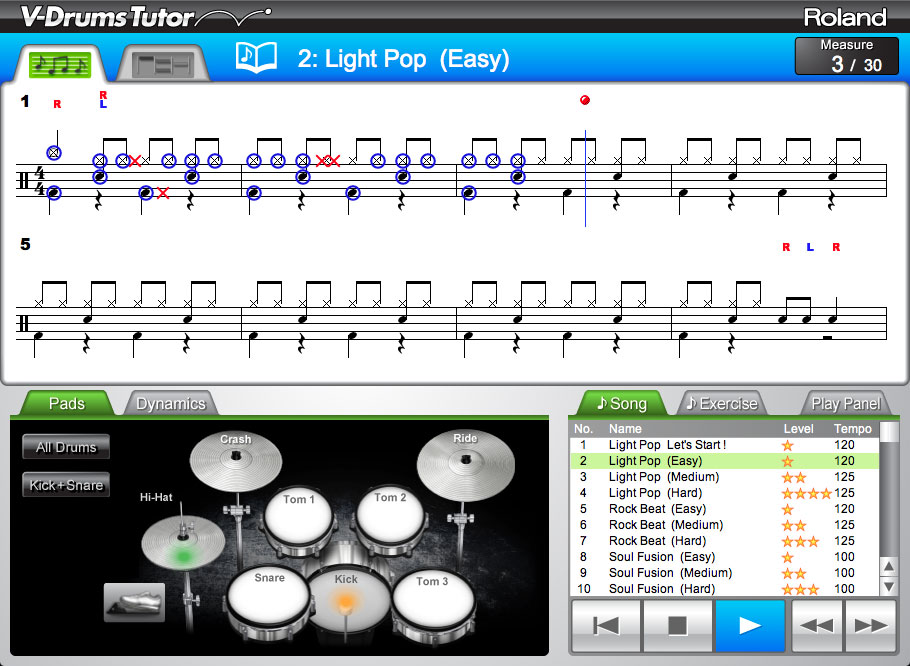
\includegraphics[scale=0.2]{dt-1_ss_main_notation_gal} 

\subsection{Current Systems}

Detecting musical time is a skill which is not only a fundamental musical skill [1] but also something that can seemingly come naturally to humans, the majority being able to analyse and reproduce discrete metrical stuctures of a piece of music [2]. Producing algorithms to replicate this nature human ability is probably first attempted by Longuet-Higgins [1], where he began to consider that rhythm as a binary tree with each node representing a note or rest. This theory developed into a system which would use a static tolerence limit on how much a the downbeats varied and enabling the perceived tempo to be adjusted accordingly [add longuet references]. Since Longuet-Higgins first work there have been a number of different approaches to beat detection in audio, M. Goto and Y. Muraoka created a system which would learn the frequencies of the bass drum and snare drum, in order to then detect events triggered by these instruments during a piece of music [Goto & muroaka]. In 2001 Simon Dixon presented a system which uses processed a piece of audio in order to generate a tempo hypotheses at various metrical levels, multiple agents were then employed to find the sequence of beat times which best matched the salient rhythmic events which were originally detected.

The majority of the audio beat detection systems developed to date rely on an onset detection function, where an audio onset is considered to be the beginning of each music note within a piece of music[https://en.wikipedia.org/wiki/Onset_(audio)] and therefore can be used to find time-locations within all sonic events in a piece of music [https://en.wikipedia.org/wiki/Onset_(audio)].

systems developed to perform beat tracking and temporal analysis with the majority using the ``surfboard'' method first described by schloss which observed the peaks of sound energy within a piece of music in order to discern the beat locations and temporal information [schloss]. 

This method however was not considered accurate enough to fully replicate the skill of a trained musician at beat detection, it was soon recognised that onset detection would play a fundamental part in any future beat detection algorithms. Where the an indicator of a new onset is seen as ``an increase in energy (or amplitude) within some frequency band(s)'' [4].

Need to include the different types of 

Due to the rapidly expanding research being carried out on beat detection, in 2005 the 1st annual Music Information Retrieval Evaluation eXchange (MIREX) was held. MIREX has been set up as a contest with the goal of comparing state-of-the-art algorithms and music information retrieval [MIREX website]. The topics to be evaluated were proposed by the participants and in the first year, three of the nine topics concerned beat detection (Audio Drum Detection, Audio Onset Detection and Audio Tempo Extraction).  

Find the reference regarding how much work has been done in this field

Light version of beatroot and DWT

Needs to add history of all the work carried out on audio analysis with an emphasis on tempo detection

Beat detection and tempo analysis is a fundamental skill honed by musicians and in particularly drummers, their ability to perform at a consistent tempo determines a piece of musics rhythm. 

To date, the majority beat detection software has focused mainly on the dj industry where tempo and beat matching are popular aspects to be included in modern dj programs. There are however other sectors of the music industry would find beat detection software a useful, in particular, drummers could find it an enormously useful training tool. There are currently many systems available to a drummer, 




\subsection{}

\maketitle{} \section{Aims and Objectives}
As part of my project I propose to build a real time drumbeat tempo analyser which wiill implement a variety of different wave analysis algorithms. sound energy analysis and discrete wavelet transform technologies. I will provide more details regarding the system architecture in the following sections. 

Investigate with a sole focus on drums how accurate/reliable the beatroot and discrete wavelet transform algorithms are in order to ascertain how viable a future mobile metronome and drum tempo training application would be.



\subsection{Proposed Architecture}
In order to function sufficiently the system will need to encompass the following features:

The open sourced JWave library includes a Java implementation of the Discrete Wavelet Transform (DFT) algorithm.

Beatroot has 

\begin{itemize}
\item Provide real time feedback to player on the tempo of the current drum beat.
\item 
\item Sufficent signal processing, the solution will need to process the audio in appropirate durations 
\end{itemize}




\maketitle{} 
\section{Development Plan for the Solution}

\subsection{Overview of External Libraries}



Adapt beetroot library in order to allow for efficient real time analysis

implement matlab algorithm in scala/java

develop audio capture and processing system 

\maketitle{} 
\section{Project Schedule}

\begin{table}[H]
\caption{Project Timeline} 
\centering
\begin{tabular}{ | L |c| L |}
\hline\hline 
Dates & Task & Priority\\ [0.5ex]
\hline 
Jun 13 - Jun 19 & Integrate APIs and external libraries & MUST
\end{tabular}
\label{stages} 
\end{table}

\maketitle{} 
\section{References}
http://www.roland.co.uk/blog/exploring-roland-dt-1-v-drums-tutor-software/


\end{document}
